\begin{refsection}[operations/uno/group.bib]
\nocite{*}
\chapter{System Operations and Development Team}

\section{Members}

\begin{itemize}
  \item[] Atsuya Uno (Team Head)
  \item[] Hitoshi Murai (Research \& Development Scientist)
  \item[] Motoyoshi Kurokawa (Research \& Development Scientist)
  \item[] Keiji Yamamoto (Research \& Development Scientist)
  \item[] Fumio Inoue (Research \& Development Scientist)
  \item[] Yuichi Tsujita (Research \& Development Scientist)
  \item[] Mitsuo Iwamoto (Technical Staff)
  \item[] Katsufumi Sugeta (Technical Staff)
\end{itemize}


\section{Research Activities}
K computer, a distributed-memory parallel computer comprising 82,944 computing nodes, has played a central role in the High Performance Computing Infrastructure (HPCI) initiative granted by the Ministry of Education, Culture, Sports, Science and Technology.
The HPCI has achieved the integrated operation of the K computer and other supercomputer centers in Japan and has enabled seamless access from user machines to a cluster of supercomputers that includes the K computer.
Moreover, the HPCI has provided large-scale storage systems that are accessible from all over Japan.

The System Operations and Development Team (SODT) has conducted research and development on the advanced management and operations of the K computer.
While analyzing operational statistics collected during shared use, the SODT has improved the system configuration, including aspects involving job scheduling, the file system, and user environments.
As an example, achieving higher system utilization is very difficult, because the K computer must simultaneously process various sizes and types of jobs.
The SODT has responded flexibly to user requests and analyzed operational status, thereby realizing a high level of utilization of approximately 75\% in the fiscal year 2015 (FY2015).
Moreover, the SODT has developed tools that improve the usability of the K computer.
The SODT has also helped users manage the K computer and utilize the K computer resources effectively by improving the system software.
Note that this support was achieved together with the software development team.

In FY2015, we primarily implemented improvements to operational issues.
In particular, we addressed the performance degradation issue of the file system and the long waiting times of some jobs.
In addition, we implemented a performance monitoring system for the global file system (GFS) and local file system (LFS).
As for electric power use, we developed an automatic emergency job-stopping method and implemented a system to estimate future electric power needs.

\section{Research Results and Achievements}
Figure~\localref{fig:usage} shows resource usage details for FY2015.
As shown in the figure, we achieved approximately 75\% node usage, which is the same as FY2014.
Each project had appropriate computing resources for a year, and these resources were divided into the following two terms : (1) from April to September and (2) from October to March.
In FY2015, node usage during the first term was 71\%, whereas the usage during the second term was 80\%.
In contrast, node usage per term in FY2014 was 79\% and 72\%, respectively.
Because many new projects were initiated in FY2015, utilization of the first term (especially in April and May) decreased.

\begin{figure}
\centering
  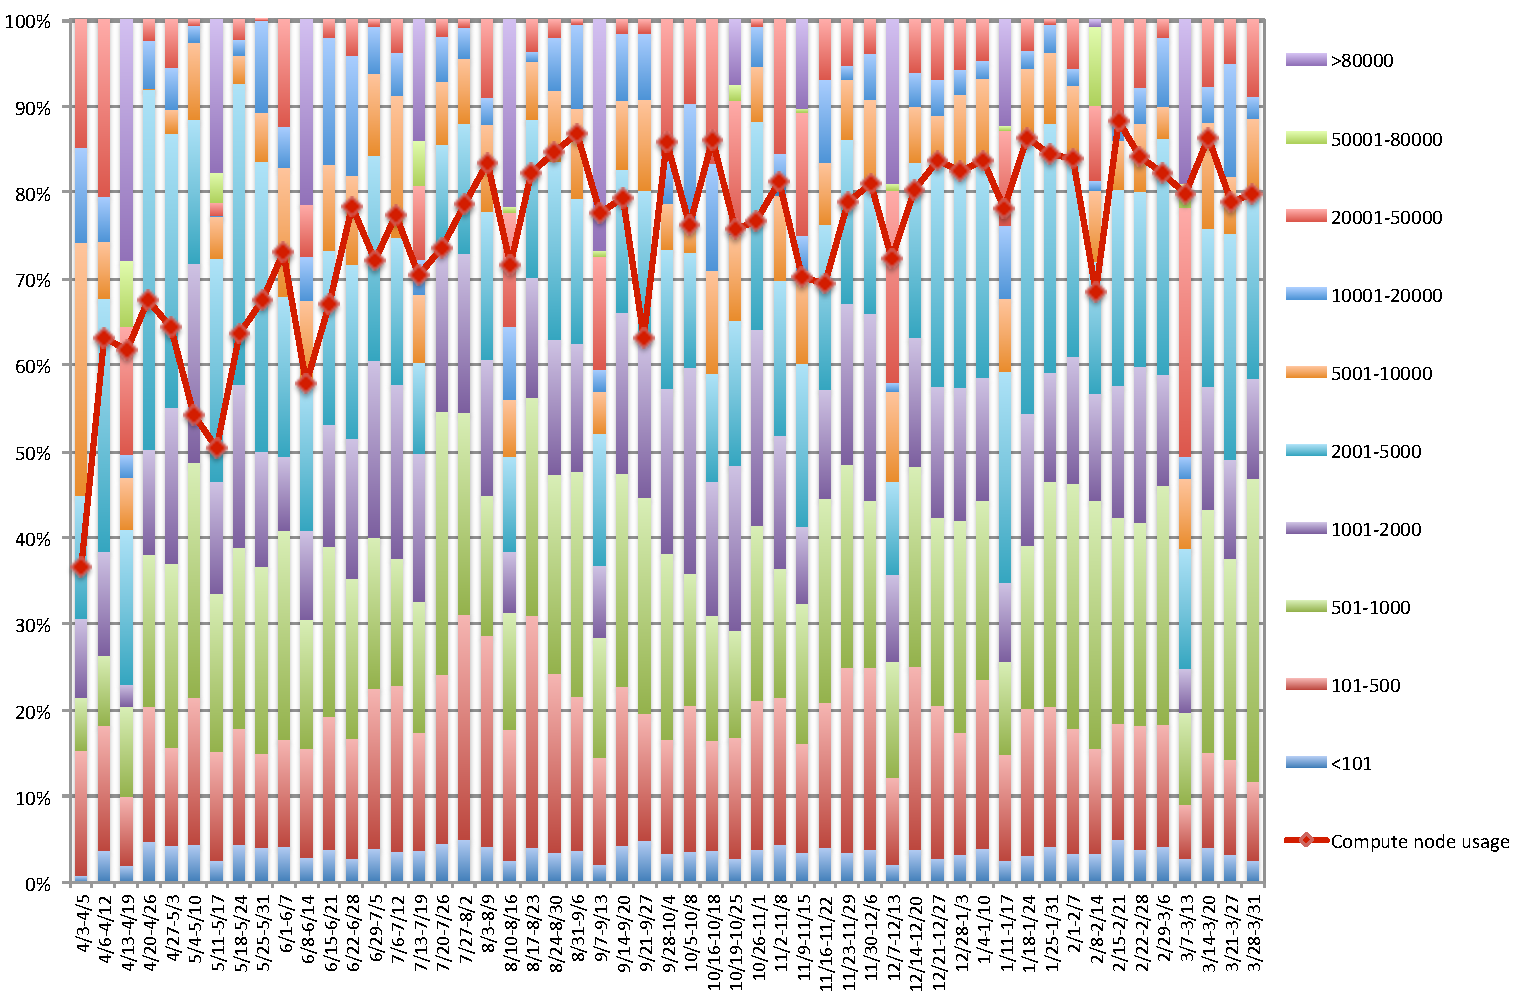
\includegraphics[width=0.95\textwidth,keepaspectratio]
  {operations/uno/images/details_of_resource_usage.pdf}
  \caption{Resource usage in FY2015}
  \locallabel{fig:usage}
\end{figure}

\subsection{Analysis and improvements of operational issues}

\subsubsection{Shortening job waiting times}
Figure~\localref{fig:waiting} shows the average waiting times of large jobs (i.e., 12289--36864 nodes) in both FY2014 and FY2015.
To consume remaining computing resources before they expired, users tended to submit many jobs at the end of each term, the average waiting times in September and March were substantially longer than those of other months.
In FY2014, job congestion occurred in August and September; however, in the second term of FY2015, they occurred from December.
In addition, average waiting times for FY2015 were longer than those of FY2014.
We therefore analyzed job scheduling and found that the following two factors impacted long waiting times.

\begin{figure}
\begin{minipage}{0.5\hsize}
\centering
  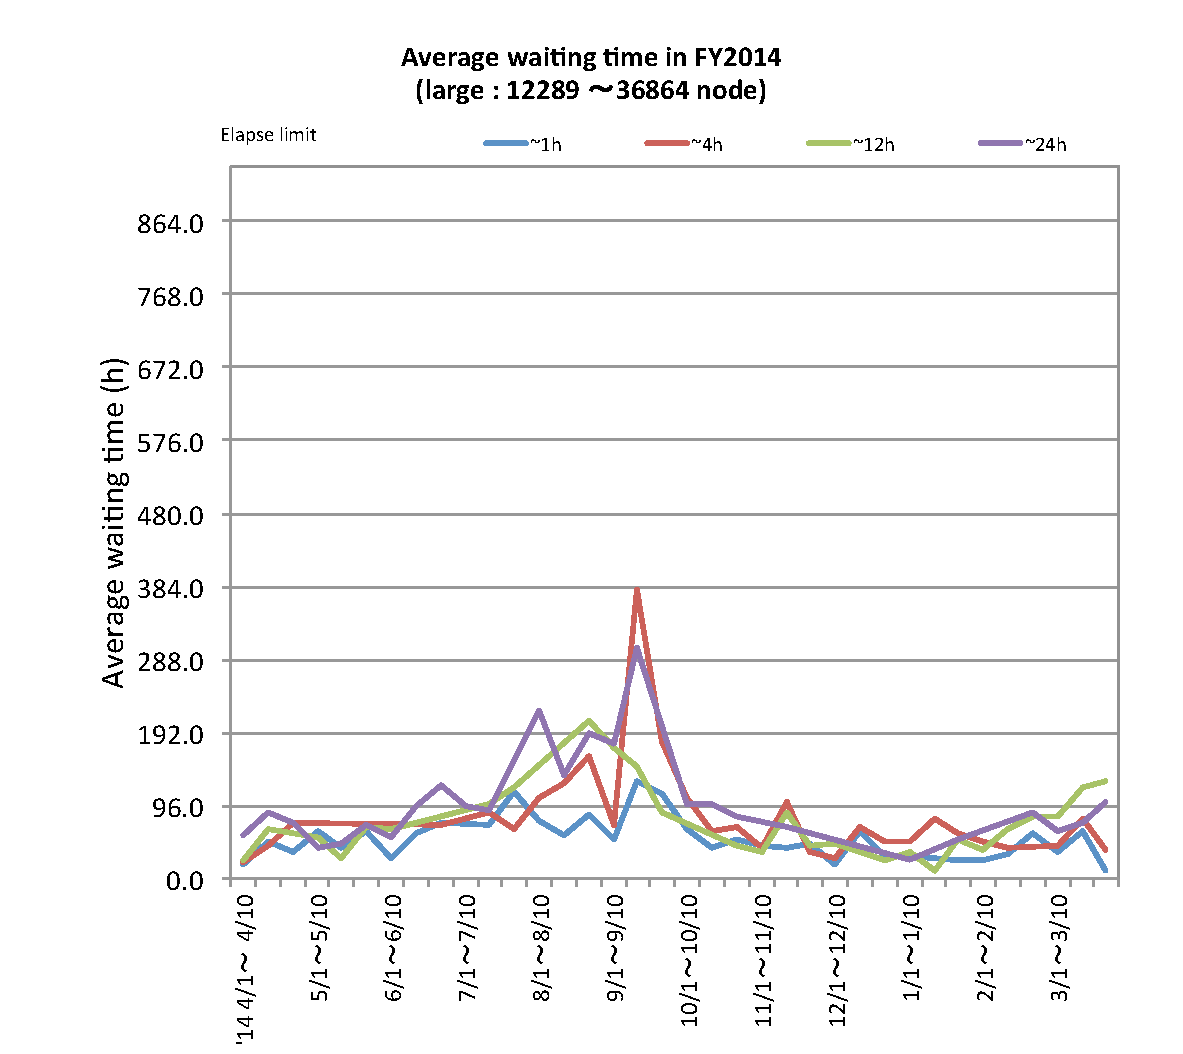
\includegraphics[width=0.95\hsize,keepaspectratio]
  {operations/uno/images/waittime2014.pdf}
\end{minipage}
\begin{minipage}{0.5\hsize}
\centering
  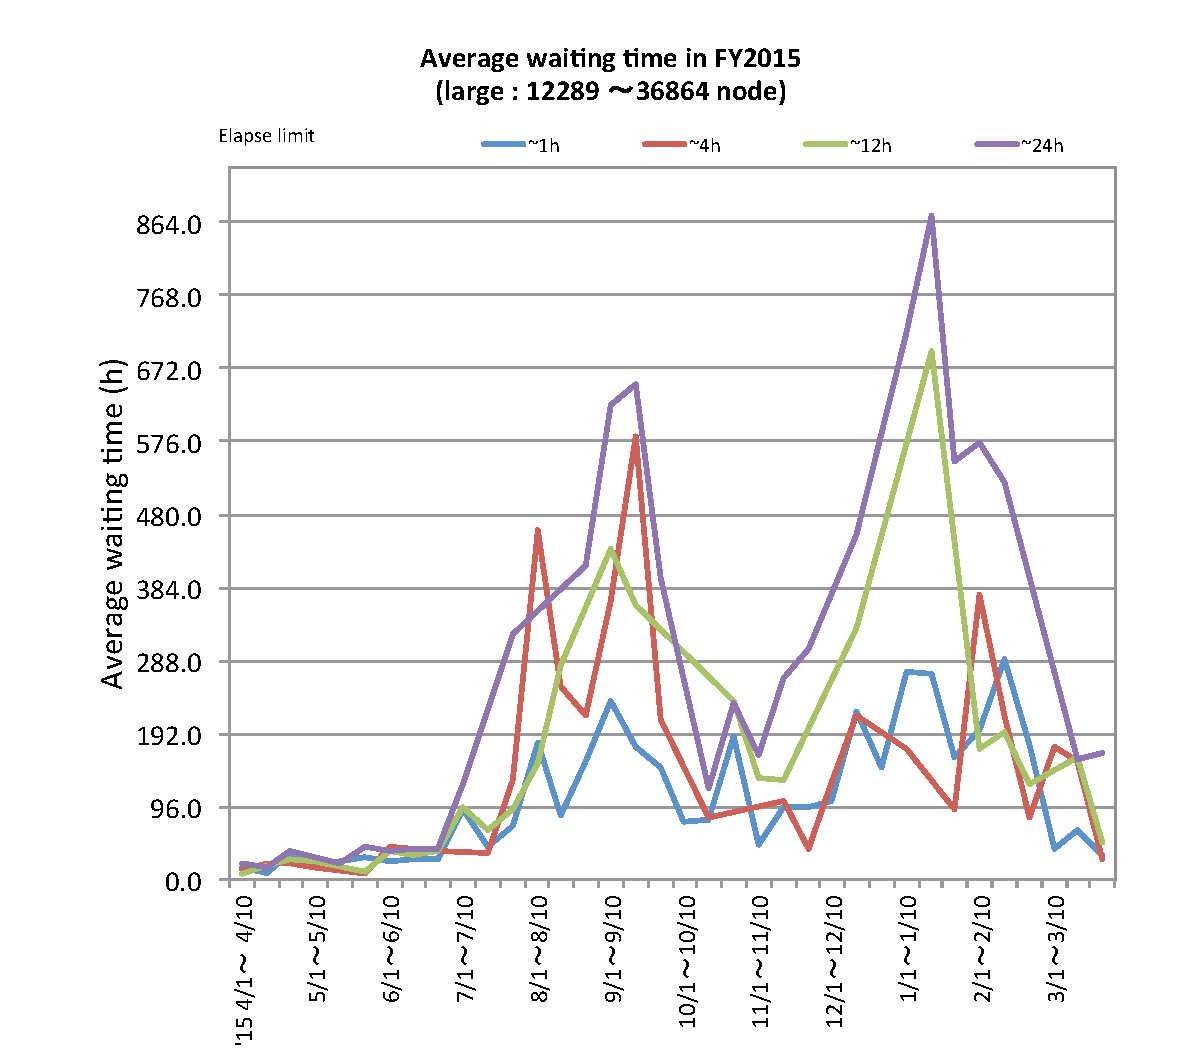
\includegraphics[width=0.95\hsize,keepaspectratio]
  {operations/uno/images/waittime2015.pdf}
\end{minipage}
  \caption{Average waiting times in FY2014 and FY2015}
  \locallabel{fig:waiting}
\end{figure}

\begin{enumerate}
  \item Influence of higher-priority jobs (prior/semiprior job)

From FY2014, we provide a priority use system by which users can run a job at a higher priority than normal jobs.
Figure~\localref{fig:wait_job} shows the number of higher-priority jobs per month.
As is evident in the figure, the number of priority jobs in FY2015 was greater than that of FY2014.
Normal priority jobs, especially, large-scale jobs, are impacted by these higher-priority jobs.
In February 2016, we therefore changed the region used by higher-priority jobs to a region that may not inhibit the execution of normal jobs.

  \item Influence of jobs specified in excess of node LFS quotas

Users specify LFS quotas when a job is submitted.
There were many jobs specified with excess node LFS quotas in FY2015.
Figure~\localref{fig:wait_lfs} shows the number of occurrences of LFS space shortages in the 10,000 or more nodes of a job.
Comparing Figure~\localref{fig:waiting} and Figure~\localref{fig:wait_lfs}, we note a correlation between waiting times and LFS space shortages.
We have therefore requested a review of node LFS quotas in order not to occurrence of LFS space shortages.
In addition, we designed a system to monitor and detect LFS space shortages.
\end{enumerate}

\begin{figure}
\begin{minipage}{0.5\hsize}
\centering
  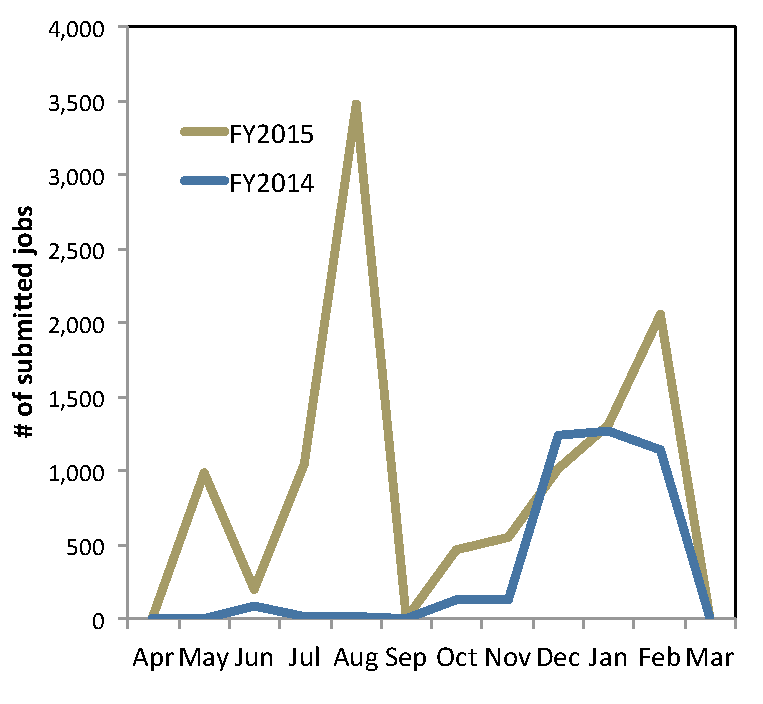
\includegraphics[width=0.95\hsize,keepaspectratio]
  {operations/uno/images/wait_job.pdf}
  \caption{Number of submission priority jobs}
  \locallabel{fig:wait_job}
\end{minipage}
\begin{minipage}{0.5\hsize}
\centering
  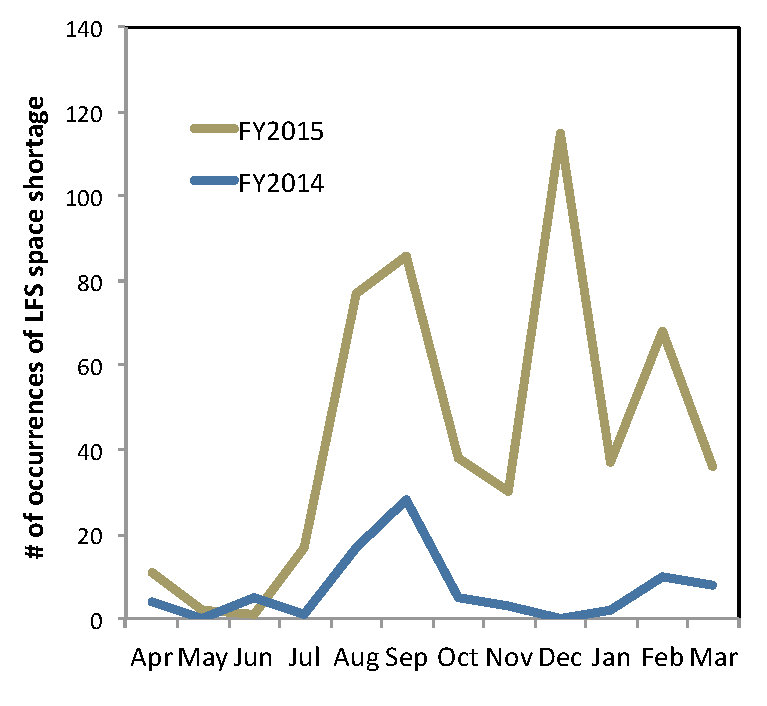
\includegraphics[width=0.95\hsize,keepaspectratio]
  {operations/uno/images/wait_lfs.pdf}
  \caption{Number of occurrences of LFS space shortages}
  \locallabel{fig:wait_lfs}
\end{minipage}
\end{figure}

\subsubsection{Response degradation problems in the GFS}
Temporary reductions in the response rates of the GFS have occurred several times.
The major factor is the load concentration on the GFS caused by large-scale staging.
Because this bandwidth is filled with access to very large files, access to other files was inhibited.

We analyzed job scheduling and found that the following two factors impacted response times.
We therefore performed the following three improvements.
Through these improvements, load balancing was achieved and response time improved.
\begin{itemize}
\item{Automatic striping of stage-out file}
\item{Processing I/O thread allocation setting for access from the front-end node and staging system}
\item{Changing the default stripe count on the GFS}
\end{itemize}

\subsubsection{Performance monitoring of the GFS and LFS}
We started to collect performance data regarding the GFS and LFS to monitor load.
We use these data to detect failures and analyze each job's I/O performance.
Every 10 min, our monitoring system collects and records the size of read and write operations.
Similarly, our system collects the number of metadata operations, such as open, close, getatter, etc.
In the future, we will evaluate the job's I/O performance using these gathered performance data.

\subsubsection{Disclosure of information to the user}
We constructed a webpage to present the following information on the K user portal.
\begin{itemize}
\item{Resource use history, including job and storage information}
\item{Detailed performance information of each job}
\item{Login history}
\item{Performance information on jobs executed by pre/post processing nodes}
\end{itemize}

\subsection{Power consumption problem}
The K computer's power consumption exceeded the given limit several times during FY2013; this is an important problem because it forces us to increase the contracted upper limit for power, thereby increasing costs, which cannot be ignored.
From FY2014, to prevent this problem, we performed a preliminary review that estimated the power consumption of each job, thereby enabling us to control the K computer's overall power consumption.
Moreover, we investigated an emergency job-stopping method based on the estimated power consumption of each job in case power consumption again exceeds the given limit.
In FY2015, we primarily worked on improvements to our emergency job-stopping method and algorithm to predict power consumption a few hours into the future.
\subsubsection{Improvements to our emergency job-stopping method}
In FY2014, the staff of the facility monitored and stopped jobs when power consumption exceeded given limits.
Because this method was manual, it took time to stop a job and was prone to human error.
In FY2015, we built a management system for the K computer that can read power information of the facilities.
When this system detects excess power use, it automatically stops the current job.
Immediate response times are required when excess power is demanded, thus automated job stopping led to further protection.
In FY2014, we used a simple approach, i.e., we selected the largest job in terms of the number of nodes as the job to be stopped.

In FY2015, we evaluated other selection methods that take into account the power consumption, number of nodes and elapsed time of the jobs.
Selecting jobs to stop is a combinatorial optimization problem; thus, we used a genetic algorithm to solve the problem.
In FY2016, we plan to operate and evaluate this emergency job-stopping system.

\subsubsection{Power consumption prediction}
To prevent excess power consumption, the cogeneration system (CGS) is useful to temporarily increase power supply.
Two CGS of 5 MW are operated alternately in AICS.
If two CGSs are operated simultaneously when excess power is expected, we can avoid the excess power.
Because CGS takes 1--2 hours to initiate, we must expect excess power to be demanded in a few hours.
We abandoned the full-time operation of two CGSs, because fuel costs increasesd.
We examined our prediction method regarding power fluctuations after a few hours.
According to job statistics, many users execute jobs repeatedly with the same number of nodes.
Moreover, 80\% of users executed jobs with at most nine patterns in terms of the number of nodes.

We therefore implemented a power forecast system that estimates the power of a scheduled job using power history of already-executed jobs.
Figure~\localref{fig:forecast} presents an example of predicted power usage at 10:30 AM, showing data from 12 hours before until 12 hours after 10:30 AM.
In other words, the center of the figure represents now.
The past shows the record of power, while the future shows predicted power usage.
The dashed lines in the figure indicate the upper and lower limits of the predicted power plus statistical prediction errors.
In FY2016, we plan to improve prediction accuracy by using machine learning and evaluate our emergency job-stopping system.
In addition, we plan to study optimal operation methods of the CGS using our prediction results.

\begin{figure}
\centering
  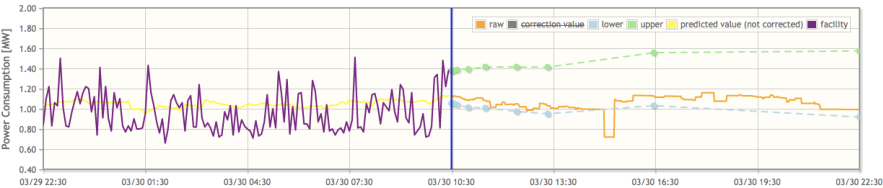
\includegraphics[width=0.95\textwidth,keepaspectratio]
  {operations/uno/images/forecast.pdf}
  \caption{Power Consumption Forecast at 10:30 AM}
  \locallabel{fig:forecast}
\end{figure}

\subsection{User support}
The K computer had approximately 170 groups and 1,900 users in FY2015.
The total number of HPCI users and AICS researchers were approximately 1,600 and 300, respectively.
The number of daily active users was approximately 150.

We supported users through the K support desk, providing users with technical information on the K computer, including information regarding its system environment, system tools, software libraries.
In addition, we performed user registrations, failures investigation and software installation, etc.
Our consulting services were offered together with the software development team.
Figure~\localref{fig:support} present the number of issues addressed in FY2015, showing the number of new issues in FY2015 to be approximately 230; the number of resolved issues was approximately 220.
The number of new issues in FY2013 and FY2014 were approximately 230 and 170, respectively.

\begin{figure}
\centering
  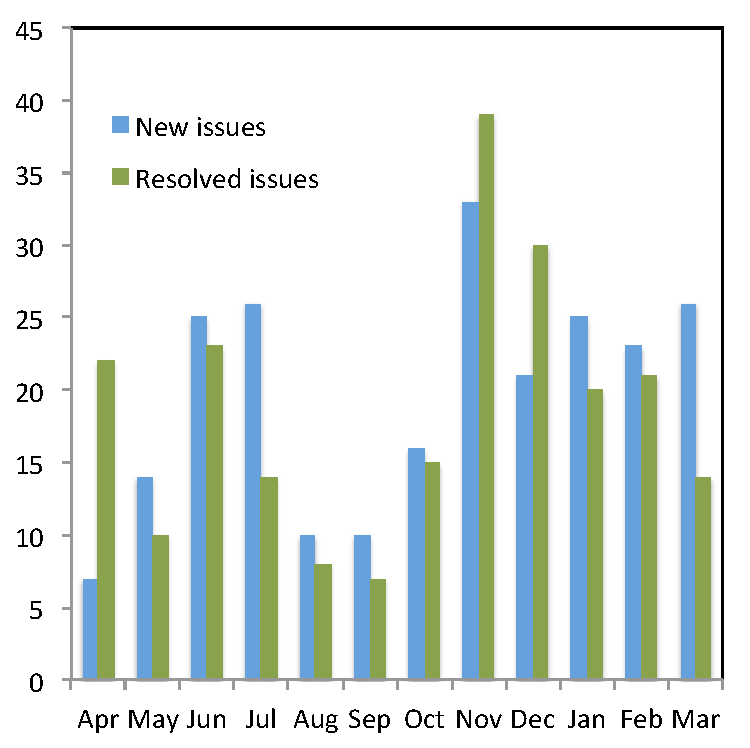
\includegraphics[width=0.4\textwidth,keepaspectratio]
  {operations/uno/images/ai.pdf}
  \caption{Number of issues addressed in FY2015}
  \locallabel{fig:support}
\end{figure}

\section{Schedule and Future Plan}
In FY2015, we primarily performed improvements on operational issues.
We analyzed the operational status, identified a variety of issues, and made improvements in these areas.
To implement these improvements, we constructed a log-gathering environment and a database.
In the next fiscal year, we are scheduled to publish the compiler, which supports the new standard.
We continue to improve the user environment and provide user support.
Moreover, we continue to address the K computer's power consumption problem.

%%% DO NOT EDIT BELOW

\section{Publications}

%\printbibliography[keyword=journal, heading=subbibliography, title={Journal Articles}, prefixnumbers={1-}, resetnumbers=true]
%\printbibliography[keyword=proceedings, heading=subbibliography, title={Conference Papers}, prefixnumbers={2-}, resetnumbers=true]
%\printbibliography[keyword=invited, heading=subbibliography, title={Invited Talks}, prefixnumbers={3-}, resetnumbers=true]
%\printbibliography[keyword=poster, heading=subbibliography, title={Posters and Presentations}, prefixnumbers={4-}, resetnumbers=true]
%\printbibliography[keyword=deliverable, heading=subbibliography, title={Patents and Deliverables}, prefixnumbers={5-}, resetnumbers=true]

\printbibliography[keyword=journal, heading=subbibliography, title={Journal Articles}, resetnumbers=true]
\printbibliography[keyword=proceedings, heading=subbibliography, title={Conference Papers}]
\printbibliography[keyword=invited, heading=subbibliography, title={Invited Talks}]
\printbibliography[keyword=poster, heading=subbibliography, title={Posters and Presentations}]
\printbibliography[keyword=deliverable, heading=subbibliography, title={Patents and Deliverables}]

\end{refsection}
